%!TEX root = ../Report.tex

In this chapter of the report, we discuss the results of the experiments and their ramifications. The structure of this section mirrors that of the experiments section, so that the first results discussed will be the first experiment detailed in chapter \ref{chapter:experimental_methodology_and_program}.



\section{Experiment Results}



\subsection{Experiment 1 - Metrics Collection Overhead}

In experiment 1, we investigated our method for collecting metrics about the system adds any significant overhead that we must take into account in assessing further experiments. Looking at the following results, particularly the percentage of total runtime, it seems that we can assume the performance difference is negligible. (*** Is 3.5\% still negligible? I could reduce it with a little work***)


\begin{figure}[H]
	\centering
	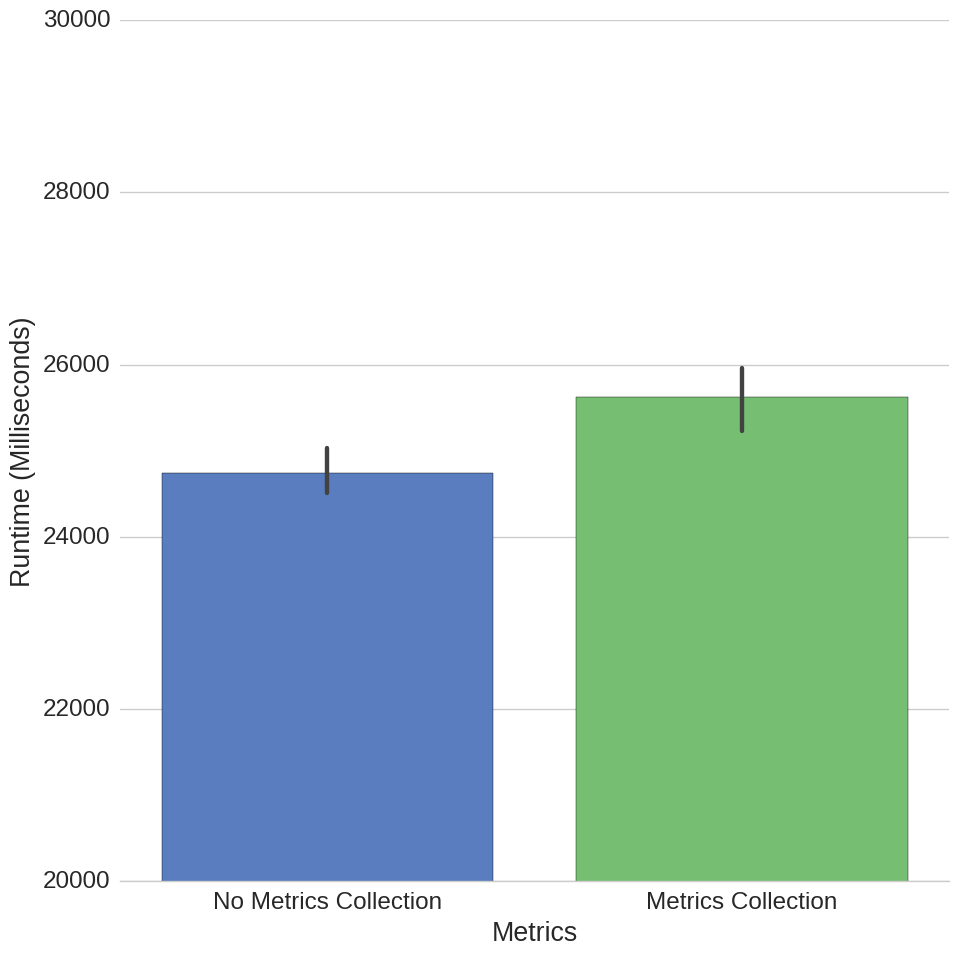
\includegraphics[width=\textwidth]{graphics/experiment1.png}
	\caption{Experiment 1 results}
	\label{fig:results_ex1}
\end{figure}

\begin{table}[H]
\centering
	\begin{tabular}{|c|c|}
		\hline
		Average delay added & 877ms \\
		\hline
		Percentage of total runtime & 3.5\% \\
		\hline
	\end{tabular}
	\caption{Experiment 1 Results Analysis}
	\label{table:results_experiment_1_results_analysis}
\end{table}

%% LaTeX2e file `ex_params/ex1_params.tex'
%% generated by the `filecontents' environment
%% from source `Report' on 2017/03/25.
%%
\begin{table}
\centering
 \begin{tabular}{|c|c|}
  \hline
  Number of tasks & 100,000 \\
  \hline
  Task Grain & 100,000 Repeats \\
  \hline
  Task Grain Distribution & Uniform \\
  \hline
  Number of CPU cores & 4 \\
  \hline
  Number of threads used & 4 \\
  \hline
  Thread pinning & Uniform \\
  \hline
  Schedule & Dynamic Chunks (Chunk Size = 1000) \\
  \hline
 \end{tabular}
\caption{Experiment 1 Parameters}
\iflabela
\label{table:evaluation_ex1_parameters}
\fi
\labelatrue
\end{table}




\subsection{Experiment 2 - Absolute Performance}

In this experiment, the total run times of three implementations are measured. One sequential implementation, a standard modern parallel implementation utilizing OpenMP, and our plastic implementation of map\_array. Our plastic implementation is running with no plasticity for the moment, and with no messaging functionality at all. This is so it is comparable to a standard parallel implementation, since the purpose of this experiment is to test our baseline performance.

Both OpenMP and our implementation are using a dynamic chunks schedule, with a chunk size of 1000.

Figure \ref{fig:results_ex2} shows us that with a single thread, our performance is similar to a sequential implementation, and as we increase the thread count, our performance scales accordingly. Overall, this shows that our implementation performs on a par with current parallel implementations, providing a good baseline performance. 



\begin{figure}
	\centering
	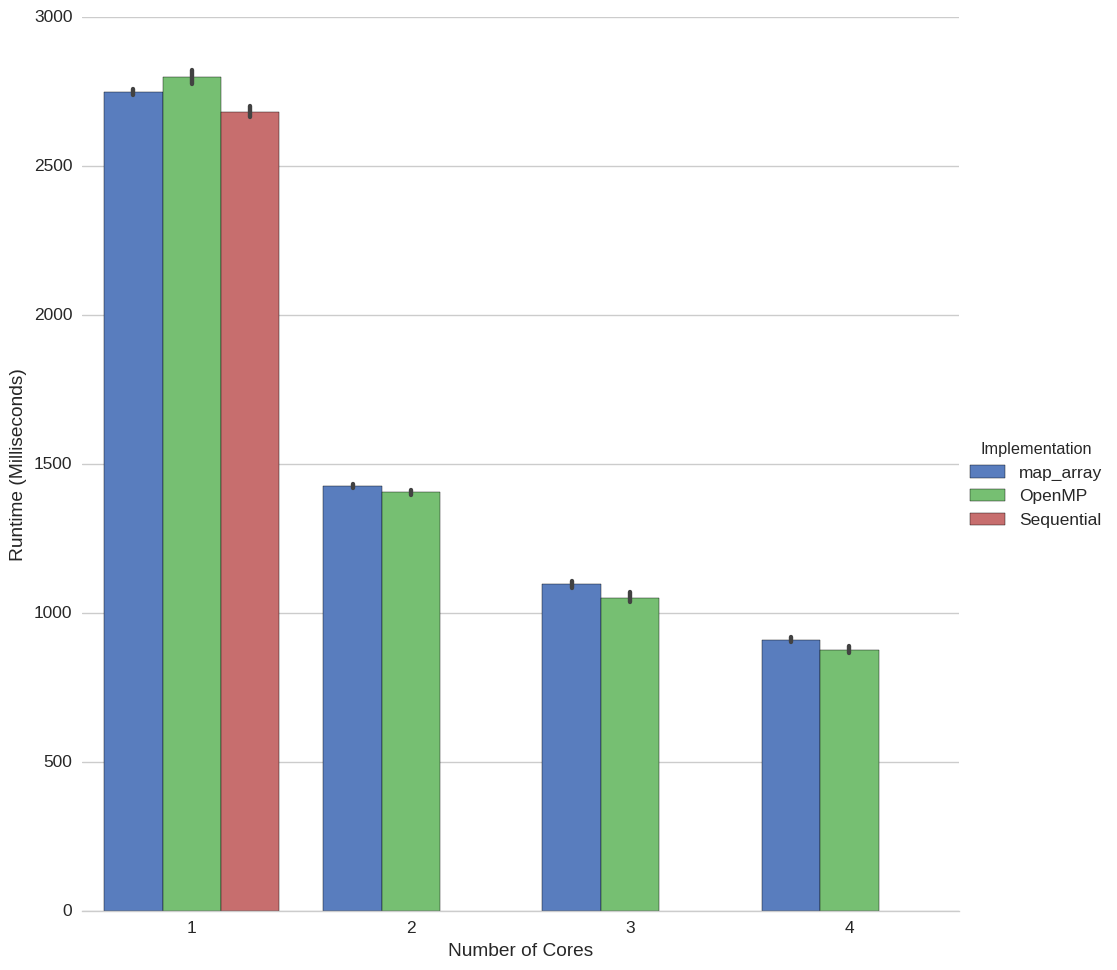
\includegraphics[width=\textwidth]{graphics/experiment2.png}
	\caption{Experiment 2 results}
	\label{fig:results_ex2}
\end{figure}

%% LaTeX2e file `ex_params/ex2_params.tex'
%% generated by the `filecontents' environment
%% from source `Report' on 2017/03/25.
%%
\begin{table}
\centering
 \begin{tabular}{|c|c|c|c|}
  \hline
  Number of tasks & 10,000 \\
  \hline
  Task Grain & 1,000,000 Repeats \\
  \hline
  Task Grain Distribution & Uniform \\
  \hline
  Number of CPU cores & 4 \\
  \hline
  Number of threads used & \specialcell{1, \\ 2, \\ 3, \\ 4} \\
  \hline
  Thread pinning & Uniform \\
  \hline
  Schedule & Static \\
  \hline
 \end{tabular}
\caption{Experiment 2 Parameters}
\iflabelb
\label{table:evaluation_ex2_parameters}
\fi
\labelbtrue
\end{table}




\subsection{Experiment 3 - Plasticity And Contention Aware Scheduling Framework Overhead}

This experiment was designed to assess the amount of overhead added by plasticity and the contention aware scheduling framework. The results are strange, because we would expect the runtime to only increase with the added overhead, but we have two cases where the runtime decreases. 

With our smallest array size of 1000, we see an increase of 2ms, which is 2.7\% of the total runtime. These results are very close, and within the margin of error. 

Our other results both show a decrease in runtime, again both within the margin of error. Possible reasons:

(*** I suspect this weirdness may be down to different circumstances when the experiments were run. Especially since the difference is most pronounced with the largest array size, since it has the largest time for things to change. Also, using a virtual machine can't help. I'll see if I can run them on another machine. ***)

The overall takeaway from this experiment, is that the added overhead is negligible when measuring the total runtime, with a wide selection of array sizes.



\begin{figure}[H]
	\centering
	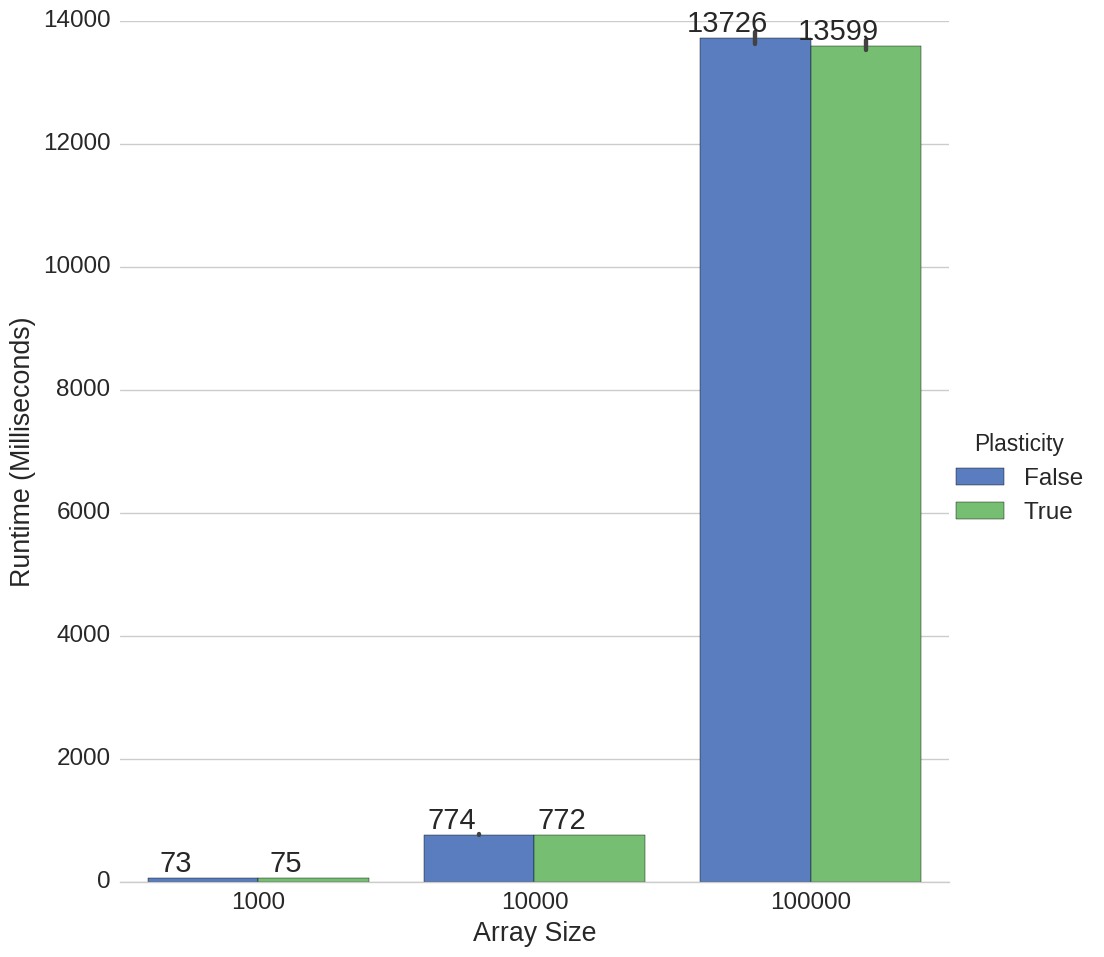
\includegraphics[width=\textwidth]{graphics/experiment3.png}
	\caption{Experiment 3 results}
	\label{fig:results_ex3}
\end{figure}

\begin{table}[H]
\centering
	\begin{tabular}{|c|c|}
		\hline
		Average delay added (Few tasks) & 2ms \\
		\hline
		Percentage of total runtime (Few tasks) & 2.7\% \\
		\hline
		\hline
		Average delay added (Med. tasks) & -2ms \\
		\hline
		Percentage of total runtime (Med tasks) & N/A \\
		\hline
		\hline
		Average delay added (Many tasks) & -127ms \\
		\hline
		Percentage of total runtime (Many tasks) & N/A \\
		\hline
	\end{tabular}
	\caption{Experiment 3 Results Analysis}
	\label{table:results_experiment_3_results_analysis}
\end{table}

%% LaTeX2e file `ex_params/ex3_params.tex'
%% generated by the `filecontents' environment
%% from source `Report' on 2017/03/25.
%%
\begin{table}
\centering
 \begin{tabular}{|c|c|}
  \hline
  Number of tasks & 100,000 10,000 1,000 \\
  \hline
  Task Grain & Medium \\
  \hline
  Task Grain Distribution & Uniform \\
  \hline
  Number of CPU cores & 4 \\
  \hline
  Number of threads used & 4 \\
  \hline
  Thread pinning & Uniform \\
  \hline
  Schedule & Dynamic Chunks \\
  \hline
 \end{tabular}
\caption{Experiment 3 Parameters}
\iflabelc
\label{table:evaluation_ex3_parameters}
\fi
\labelctrue
\end{table}




\subsection{Experiment 4 - Schedule Choice Importance}

This experiment was designed to highlight the importance of choosing the correct schedule, and how we can benefit from runtime plasticity. We have a biased set of tasks, (first quarter of which are large tasks, the rest small,) meaning the static schedule will perform poorly, and the dynamic schedules will fare well.

This is reflected in the results, where we see the dynamic schedules perform almost three times as well as the static schedule. Also included is a case where we start with the static schedule, and then switch to dynamic chunks after five seconds. We see it perform on a par with our dynamic schedules, again greatly improving upon the static schedule.



\begin{figure}
	\centering
	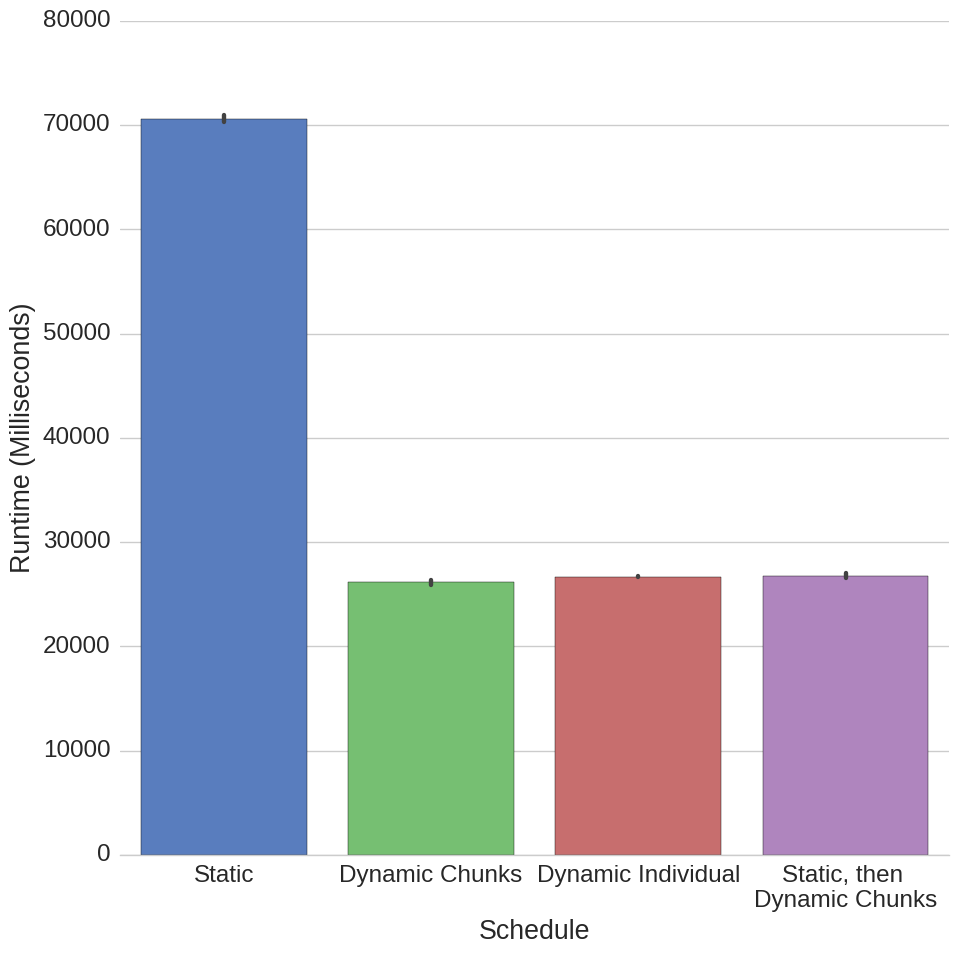
\includegraphics[width=\textwidth]{graphics/experiment4.png}
	\caption{Experiment 4 results}
	\label{fig:results_ex4}
\end{figure}

%% LaTeX2e file `ex_params/ex4_params.tex'
%% generated by the `filecontents' environment
%% from source `Report' on 2017/03/25.
%%
\begin{table}
\centering
 \begin{tabular}{|c|c|}
  \hline
  Number of tasks & 100,000 \\
  \hline
  Task Grain & Large and small \\
  \hline
  Task Grain Distribution & Biased \\
  \hline
  Number of CPU cores & 4 \\
  \hline
  Number of threads used & 4 \\
  \hline
  Thread pinning & Uniform \\
  \hline
  Schedule & \specialcell{Static, \\ Dynamic Chunks (Chunk Size = 1,000), \\ Dynamic Chunks (Chunk Size = 1) \\ Static, then dynamic chunks after 5 seconds} \\
  \hline
 \end{tabular}
\caption{Experiment 4 Parameters}
\iflabeld
\label{table:evaluation_ex4_parameters}
\fi
\labeldtrue
\end{table}




\subsection{Experiment 5 - Absolute Multiprogramming Performance}

%% LaTeX2e file `ex_params/ex5_params.tex'
%% generated by the `filecontents' environment
%% from source `Report' on 2017/03/25.
%%
\begin{table}
\centering
 \begin{tabular}{|c|c|}
  \hline
  Program 1 & \\
  \hline
  Number of tasks & 30,000 \\
  \hline
  Task Grain & 10,000,000 Repeats \\
  \hline
  Task Grain Distribution & Uniform \\
  \hline
  Number of CPU cores & 4 \\
  \hline
  Number of threads used & \specialcell{4 \\ 4, then 2, then 4} \\
  \hline
  Thread pinning & \specialcell{Loose, \\ Uniform} \\
  \hline
  Schedule & Dynamic\_individual \\
  \hline
 \end{tabular}

 \begin{tabular}{|c|c|}
  \hline
  Program 2 & \\
  \hline
  Number of tasks & 15,000 \\
  \hline
  Task Grain & 10,000,000 Repeats \\
  \hline
  Task Grain Distribution & Uniform \\
  \hline
  Number of CPU cores & 4 \\
  \hline
  Number of threads used & \specialcell{4 \\ 2} \\
  \hline
  Thread pinning & \specialcell{Loose, \\ Uniform} \\
  \hline
  Schedule & Dynamic\_individual \\
  \hline
 \end{tabular}
\caption{Experiment 5 Parameters}
\iflabele
\label{table:evaluation_ex5_parameters}
\fi
\labeletrue
\end{table}




\section{Discussion}

 ***Discuss the findings of the results, (Mention weird runtimes with many small tasks!)***